\subsubsection{Modello degli utenti}

\begin{figure}[h]
	\centering
	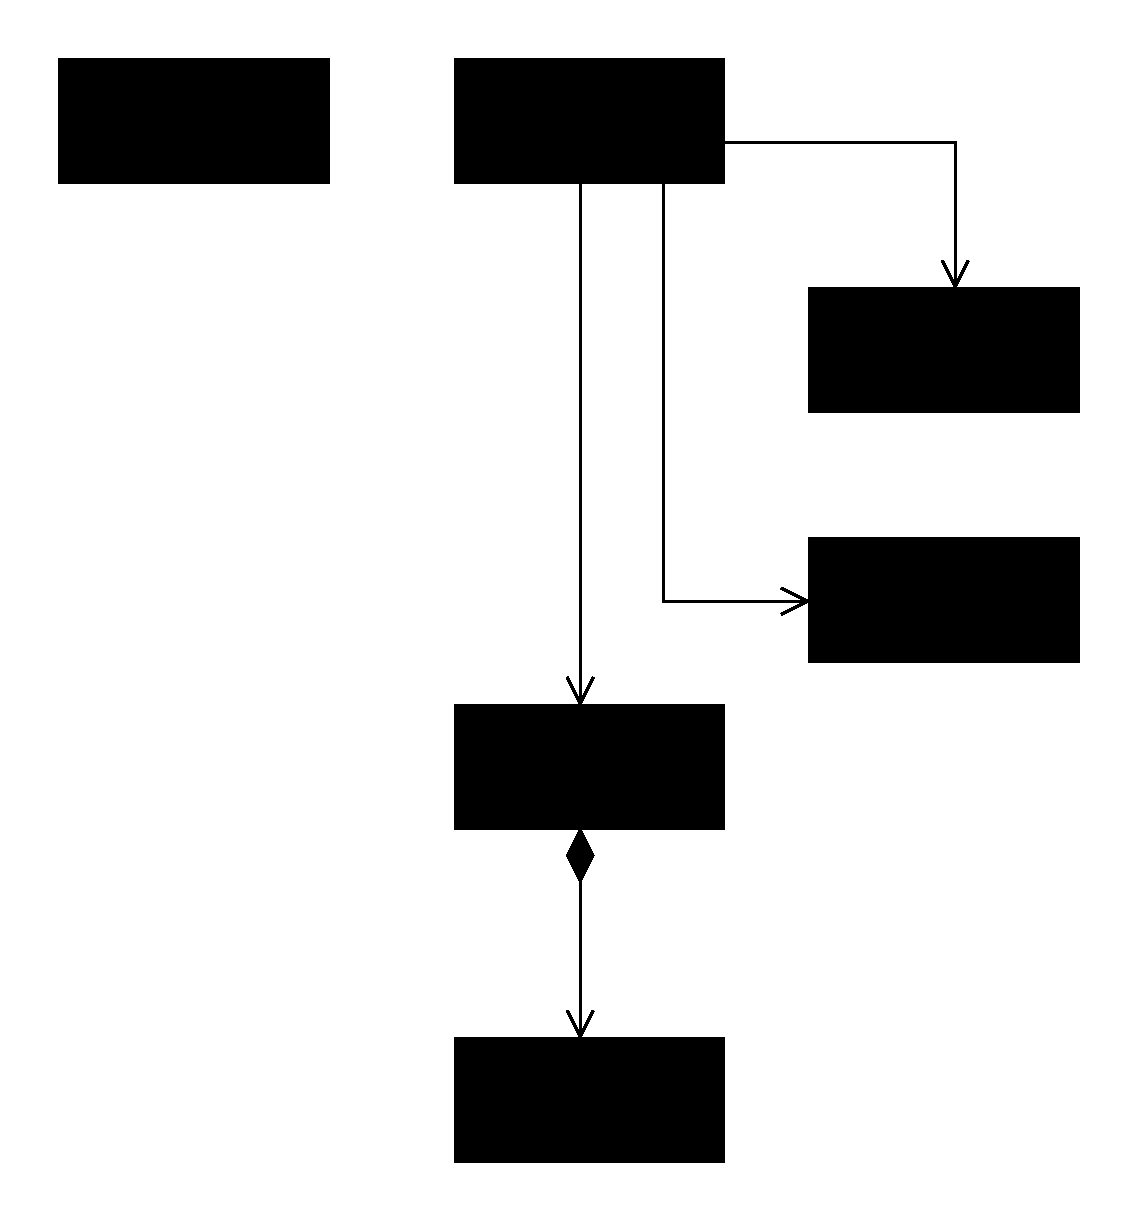
\includegraphics[width=0.6\textwidth]{user_model.eps}
	\caption{Modello degli utenti}
	\label{user_model}
\end{figure}

In figura \ref{user_model} è mostrato il modello degli utenti. \\
La classe centrale di tale modello è chiaramente \texttt{User}, che rappresenta un generico utente dell'applicazione. I tipi di utente sono rappresentati dalla enum \texttt{Role}, che può avere quattro valori:

\begin{itemize}
\item \texttt{ADMIN} (\textsl{Amministratore}). Rappresenta, appunto, l'amministratore del sistema. È l'unico che può aggiungere altri utenti di tipo Operatore o Docente. Non è afferente ad alcun dipartimento.
\item \texttt{OPERATOR} (\textsl{Operatore}). Un Operatore gestisce le convenzioni del dipartimento a cui afferisce.
\item \texttt{TEACHER} \textsl{Docente}. Il Docente può consultare le proprie convenzioni e, se richiesto, allegare documenti alle stesse.
\item \texttt{GUEST}. Rappresenta l'utente non ancora loggato. Non possiede alcun permesso.
\end{itemize}

Le operazioni che un utente può svolgere sono regolate tramite un sistema di permessi, i quali sono rappresentati dalla enum \texttt{Permission}: ad ogni \texttt{Role} è associata una lista di \texttt{Permission}. Per maggiori dettagli riguardo la sicurezza, si rimanda al capitolo INSERIRE RIFERIMENTO A CAPITOLO DELTASPIKE.\\

Un utente ha quindi un attributo che ne identifica il ruolo. Vi sono poi degli attributi che lo caratterizzano (come ad esempio l'indirizzo e-mail) ed infine un attributo di tipo \texttt{Encryptor}. \\
Questa classe racchiude metodi per gestire le diverse codifiche delle password, in modo da poter utilizzare stringhe codificate in maniera differente e rendere indipendente la codifica utilizzata dall'applicazione con quella che adopera il servizio esterno che fornisce le credenziali di Ateneo. Attualmente sono supportate due tipi di codifica: MD5 (la più utilizzata da LDAP) e SHA (adoperata anch'essa da LDAP, ma in misura minore; inoltre rappresenta la codifica di default dell'applicazione).\\
\\

Parallelamente alla classe \texttt{User} vi è la classe \texttt{Principal}, che rappresenta un client dell'applicazione. La differenza è sottile, perché rappresentano due aspetti diversi dell'utente: la prima serve per modellare l'utente all'interno dell'applicazione, la seconda serve per gestire la navigazione dell'utente. La classe \texttt{Principal} ha quindi due caratteristiche principali:
\begin{itemize}
\item è disaccoppiata dall'implementazione del modello: gli attributi del \texttt{Principal} sono di tipo stringa e ciò consente di cambiare l'implementazione sottostante indipendentemente dal \texttt{Principal}
\item è sicura, perché non contiene proprietà sensibili dell'utente (come ad esempio la password).
\end{itemize}



